\chapter{Case of study} \label{case}

In this chapter we present the relevant experiments that were done to
test the proposed method. Subsequently, it shows the implementation of
the method in a restaurant recommender system used as case of study, 
the context was integrated into the recommender system when   
we consider the contextual factors. A wide explanation of the system  
interfaces and its functionality is explained also.

\section{Experimental settings} 

In this particular experimental scenario, the basic guidelines 
proposed in Adomavicius  \cite{adomavicius2011context} are followed,  
and they are briefly explained next. 
\begin{itemize} 
\item \textbf{Hypothesis:} before running the experiment we must form
an \textit{hypothesis}. It is important to be concise and restrictive
about this hypothesis, and design an experiment that tests the
hypothesis. For example, an hypothesis can be that  \textit{algorithm
A} predicts better user ratings than  \textit{algorithm B}.  In that
case, the experiment should test the prediction accuracy, and not
other factors.
\item \textbf{Controlling variables:} when comparing a few candidate
algorithms on a certain hypothesis, it is important that all
\textit{variables} that are not tested will stay fixed. For example,
suppose that we wish to compare the prediction accuracy of movie
ratings of  \textit{algorithm A} and \textit{algorithm B}, that both
use different collaborative filtering models.
\item \textbf{Generalization power:} when drawing conclusions from
experiments, we may desire that our conclusions generalize beyond the
immediate context of the experiments. When choosing an algorithm for a
real application, we may want our conclusions to hold on the deployed
system, and generalize beyond our experimental data set. Similarly,
when developing new algorithms, we want our conclusions to hold beyond
the scope of the specific application or data set that we experimented
with. It is important to understand the properties of the various data
sets that are used. Generally speaking, \textit{the more diverse the
data used, the more it can generalize the results}.
\end{itemize} 

\subsection{Off-line experiments} 

An off-line experiment is performed using a pre-collected dataset
of users' selections or ratings. By using this dataset we try to simulate
the behavior of users that will interact with the recommender system. \\ In
doing so, it is assumed that the user behavior when the data was collected
will be similar enough to the users' behavior when the recommender
system is deployed, so that we can make reliable decisions based on
the simulation.  Off-line experiments are attractive because they
\textit{require no interaction with real users}, and thus it allows to compare
a wide range of candidate algorithms at a low cost. \\ The downside is
that it can answer a very narrow set of questions, typically questions
about the prediction of an algorithm. The goal of the off-line
experiments is to filter out inappropriate  approaches, leaving a
relatively small set of alternatives algorithms for subsequently to be
tested for the more costly user studies or on-line
experiments  \cite{adomavicius2011context}.\\
The next sections show a comprehensive description of the 
experimental setup for experiments, as well as results obtained 
in the experiments. Each method was tested using contextual 
datasets in the domain.  This chapter ends with the  
description of the functionality of the prototype used to 
validate the method utilized in the experiments.

\section{Restaurants recommendations} \label{restaurants}

In earlier implementations of the context-aware recommender system  
several experiments were done to test the behaviour of algorithms 
and the performance in the proposed method. 
For the experiment the proposed hypothesis is \textit{The accuracy of 
recommendations is improved using context factors in the 
recommendation process}. 
\begin{figure*}
\centering
\captionsetup{font=footnotesize}
\setlength\fboxsep{0pt}
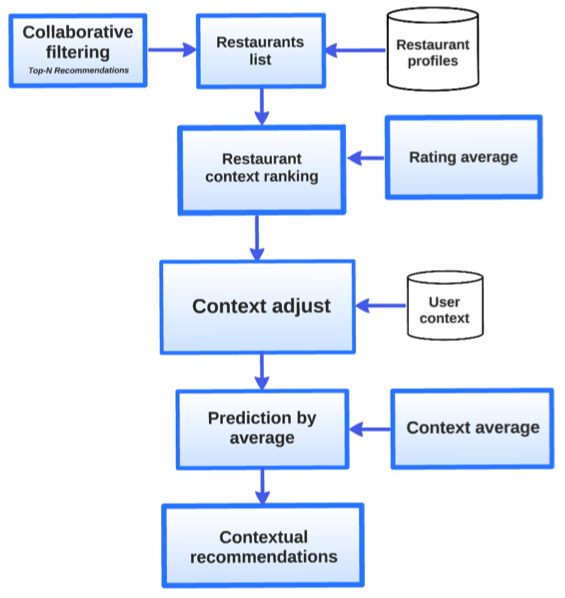
\includegraphics[width=0.50\textwidth]{img/posfil.png}
\caption{The post-filtering approach for Tijuana restaurants.}
\label{fig:postfiltering}     
\end{figure*}
To validate the hypothesis the next test was realized.
A first experiment described in  \cite{ramirez2013restaurant}, presents a  
contextual recommender system using the post-filtering approach and 
collaborative filtering technique in a restaurant domain. 
Collaborative filtering works to get a Top-N list utilized to adjust it in 
the context. \\
Later, the Top-N list is obtained and the restaurants are adjusted to 
make ranking of restaurants  in the current context. Post-filtering is
based on the average  of ratings in a specific context, so prediction
is made with: 1) \textit{the average} that a restaurant has in the
current context (that is the  mean of user ratings) and 2)  
 \textit{the rating} predicted by the collaborative filtering algorithm.\\ 
Top-N list contains the restaurants with highest predictions, 
so each restaurant is adjusted for the user's context and listed in 
contextual recommendations; the process is depicted in 
Figure  \ref{fig:postfiltering}.

\begin{table}
\small
\captionsetup{font=footnotesize}
\caption{Questionnaire applied to collect contextual dataset.}
\label{tab:questions} 
\centering
\small
\begin{tabular}{p{7cm} p{5cm} }
\hline\noalign{\smallskip}
Question & Answers \\
\noalign{\smallskip}\hline\noalign{\smallskip}
\small{1.What is your occupation?} & \small{1. Student 2.Faculty} \\ \hline  
\small{2.According to your priority, order by importance the features 
you consider when you choose to visit a restaurant.} & 
\small{1.Installation/decoration 2.Prices 3.Service 4.Dishes
5.Atmosphere 6.Location} \\ \hline  
\small{3.What devices do you use} &
\small{1.Smartphone 2.Tablet 3.Laptop 4.PC} \\ \hline   
\small{4.What Operating System do you use?} & 
\small{1.Android 2.Windows 3.iOS 4.Symbian 5.Blackberry 6.Other}
\\ \hline  
\small{5.Did you use an application to search restaurants in Tijuana?} &
\small{1.Yes 2.No 3.Which one?} \\ \hline   
\small{6.Would you like to use an application of
recommender systems of Tijuana?} & \small{1.Yes 2.No} \\ \hline  
\small{7.Please, rates your favorites restaurants(without context).} & 
\small{Restaurant list} \\ \hline
\small{8.Please, rates your favorites restaurants in contextual situations.} & 
\small{Restaurant list} \\
\noalign{\smallskip}\hline
\end{tabular}
\end{table}
In order to validate the proposed approach,  data  about 
restaurant preferences of users in different contexts was used.
The study subjects were students  with a major in engineering and  
a graduate program and faculty of the Tijuana Institute of
Technology.\\ A total of \textit{50 users} answered a questionnaire; the
questions were about their preferences for nearby restaurants and the
technology most often used by them. The \textit{questionnaire} consisted 
of \textit{eigth questions} and also they were asked to rate any number 
of restaurants from a list of 40 restaurants.
Each of the restaurants chosen, was rated six times one per proposed 
context, a matrix rating with \textit{1,422 ratings} was collected. The
questions are shown in Table  \ref{tab:questions}. \\The reason for allowing
users to chose what restaurants to rate it to give them the same liberty
that they have when visiting a web or mobile application. 
\begin{figure*}
\captionsetup{justification=centering,margin=2cm,font=footnotesize}
\centering
\setlength\fboxsep{0pt}
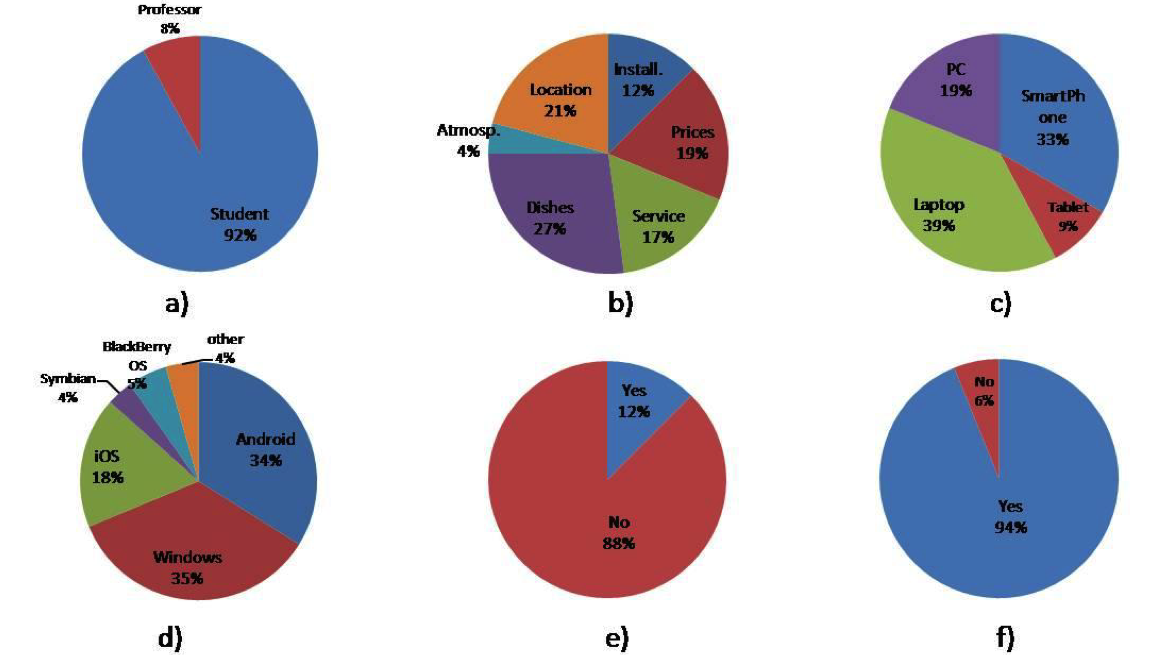
\includegraphics[width=0.8\textwidth]{img/cakes.png}
\caption{The chart cakes show the users preferences for questions from one to six.}
\label{fig:cakeschart}     
\end{figure*}
The users' answers from question one to question six are represented in
the Figure  \ref{fig:cakeschart}. Figure  \textit{\ref{fig:cakeschart}a}
represents the percentage of surveyed students and teachers;
Figure  \textit{\ref{fig:cakeschart}b}  the percentage of the element
that users consider the most important to visit a restaurant;
Figure  \textit{\ref{fig:cakeschart}c} represents the preferences of
devices when are using Internet for restaurant recommendations;
Figure  \textit{\ref{fig:cakeschart}d} represents the percentage of
operating system that often used, 
Figure  \textit{\ref{fig:cakeschart}e} shows the percentage of users 
that use the Internet to search restaurants in Tijuana; and 
Figure  \textit{\ref{fig:cakeschart}f}, shows the percentage of users 
that would like using a restaurant recommender system of Tijuana.
\begin{figure*}
\captionsetup{justification=centering,margin=2cm,font=footnotesize}
\centering
\setlength\fboxsep{0pt}
%\setlength\fboxrule{0.7pt}
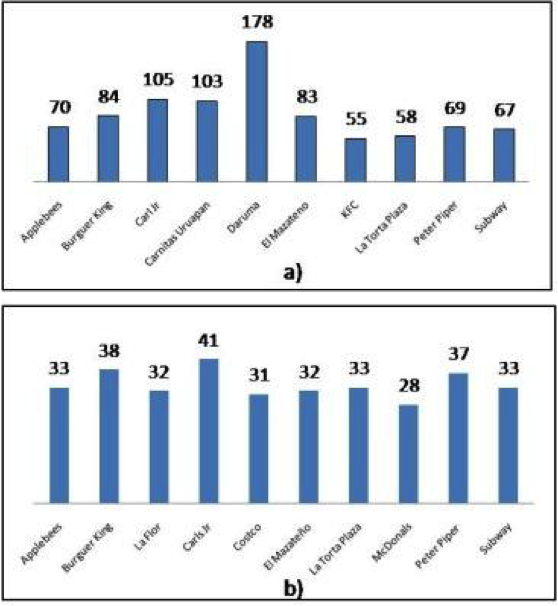
\includegraphics[width=0.55\textwidth]{img/bars.png}
\caption{The chart of users preferences for questions seven and eigth.}
\label{fig:barschart}     
\end{figure*}
\\For questions seven and eigth only the top-ten restaurants are shown,
without/with the contextual situation. In Figure  \textit{\ref{fig:barschart}a},
the favorite restaurant is \textbf{Daruma}(178 votes),  whereas in
Figure  \textit{\ref{fig:barschart}b}, \textbf{Daruma} does not appear in the
top-ten. \\When considering the context \textit{midweek}, the favorite
restaurant was \textbf{Carl's Jr.}, which appears in both graphs; this
restaurant was also the most voted in the different contexts.
Contextual recommendations of post-filtering approach depends of
context \textit{midweek} or \textit{weekend}, which is the day when
the restaurants were rated. \\Subsequently, the result of the query is
refined according to the user context; the six contexts mentioned
correspond to combinations of contextual factors shown in 
Table  \ref{tab:contextstijuana}.
\begin{table}
\small
\captionsetup{font=footnotesize}
\caption{Contextual factors considered in the questionnaire.}
\label{tab:contextstijuana} 
\centering
\begin{tabular}{p{2.0cm} p{10cm} }
\hline\noalign{\smallskip}
Contextual Factor & Context \\
\noalign{\smallskip}\hline\noalign{\smallskip}
\small{Day} & \small{1.Midweek (Monday, Thuesday,Wednesday and Thursday)
2.Weekend (Friday,Saturday and Sunday)}  \\ \hline 
\small{Place} & \small{1.School 2. Home 3.Work} \\ 
\noalign{\smallskip}\hline
\end{tabular}
\end{table}
Mean absolute error obtained was \textbf{0.5859}  in contextual
recommendations.  The observation for this result is that using a
small dataset the performance of the method proposed is limited, the
cold-start  problem affects the accuracy because of the data scarcity.

\section{Hotels recommendations} \label{hotels}

A second experiment using TripAdvisor's dataset was cunducted.  For
this case, the proposed method consisted of three algorithms  to
recommend:  \textit{fuzzy inference system}, \textit{collaborative
filtering} and \textit{content-based}. Each one uses the ratings
matrix to get recommendations.\\     The contextual recommender system
uses  \textit{post-filtering} approach  \cite{adomavicius2011context}
for adjust recommendations in context such as restaurants. 
The recommendation by popularity is  through the fuzzy inference system
depicted in Figure  \ref{fig:fis},  the fuzzy inference system
contains the variables that are involved in the process to recommend
in a human interaction, this process is the same that the recommender
system does. \\The output represents how matter each item into the
users community, i.e. if it is a popular item between users. \\ The
dataset used to evaluate the algorithm was TripAdvisor in two versions
downloaded  \cite{linkzeng}, this datasets was used in
\cite{zheng2014context} and  \cite{zheng2012differential} to  evaluate
the performance of context-aware recommender systems. \\The first
dataset contains 4669 contextual ratings, 1202 users and 1890 hotels;
the second dataset contains 14175 contextual ratings, 2731 users and
2269 hotels. 
\begin{figure*}
\captionsetup{justification=centering,margin=2cm,font=footnotesize}
\centering
\setlength\fboxsep{0pt}
\setlength\fboxrule{0.7pt}
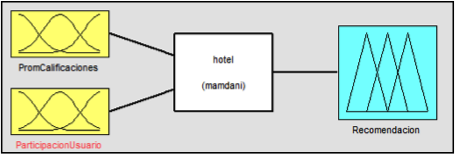
\includegraphics[width=0.75\textwidth]{img/fis.png}
\caption{Fuzzy inference system.}
\label{fig:fis}   
\end{figure*}
Data were collected of reviews online in tripadvisor.com.
There is only one context: \textit{type of trip} (family, friends,
bussines, romantic and relax).\\  The FIS has Gaussians membership
functions and are depicted in  Figure  \ref{fig:mffis}.
\begin{figure}[ht!]
   \captionsetup{font=footnotesize}
   \centering
   %%----primera subfigura----
   \subfloat[]{
        \label{fig:1a}
        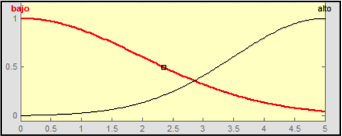
\includegraphics[width=0.42\textwidth]{img/ratingaverage.png}}
   \hspace{0.1\linewidth}
   %%----segunda subfigura----
   \subfloat[]{
        \label{fig:1b} 
        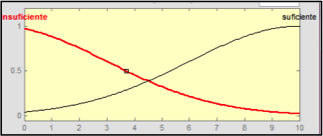
\includegraphics[width=0.42\textwidth]{img/userparticipation.png}}\\[20pt]
   %%----tercera subfigura----
    \subfloat[]{
        \label{fig:1c} 
        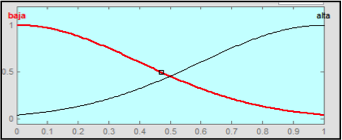
\includegraphics[width=0.42\textwidth]{img/recommendation.png}}
   \caption{Gaussian Membership functions in the input are: a) RatingAverage, 
   b) UserParticipation, and an output: c) Recommendation.}
   \label{fig:mffis} 
\end{figure}
The fuzzy inference system uses fuzzy rules to infer the inputs and 
output(a crisp value) that represents the weight of the recommendation. 
The rules are following: 
\begin{enumerate}
\item \textit{If \textbf{RatingAverage} is low and 
\textbf{UserParticipation} is insufficient then \textbf{recommendation} is low.}
\item \textit{If \textbf{RatingAverage} is low and 
\textbf{UserParticipation} is sufficient then \textbf{recommendation} is high.}
\item \textit{If \textbf{RatingAverage} is high and 
\textbf{UserParticipation} is insufficient then \textbf{recommendation} is low.}
\item \textit{If \textbf{RatingAverage} is high and 
\textbf{UserParticipation} is sufficient then \textbf{recommendation} is high.}
\end{enumerate}
Content-based uses cosine similarity to compare the binary
vectors representing the profile of each item, thereby obtaining a
numerical value that determines similarity, based on a threshold. \\   
In other words, it makes a comparison of profiles of each item to
determine the most similar to items the user has rated with highest
score, context-aware recommender system proposed has a scale 
from 1 to 5. \\
Next, the outputs of every recommender technique is represented by a
list of recommended items. Subsequently applies the context filter and
context-aware recommender system gets the final contextual
recommendations.\\  Context-aware recommender system identifies
contextual data of the user profile such as in Table  \ref{tab:2}, and
compares recommended items to filter those items that are adjusted to
the user context.  
\begin{table}[htb]
\small
\centering
\captionsetup{font=footnotesize}
\caption{Example of contextual ratings in the user profile.}
\label{tab:2}
\small
\begin{tabular}{lll}
\hline
\multicolumn{3}{c}{\textbf{User profile}} \\ \hline
Item & Rating & Context \\ \hline
La Casa del Mole & 5.0 & Midweek \\ 
Daruma           & 4.0 & Weekend \\ 
Daruma           & 5.0 & Midweek \\ 
Carl's Jr.       & 3.0 & Weekend \\ \hline
\end{tabular}
\end{table}

The context filtering is the last step before to
get the recommended items. \\The schema of architecture for context-
aware recommender system is depicted in Figure  \ref{fig:architecture}.

\begin{figure*}
\captionsetup{font=footnotesize}
%\captionsetup{justification=centering,margin=2cm}
\centering
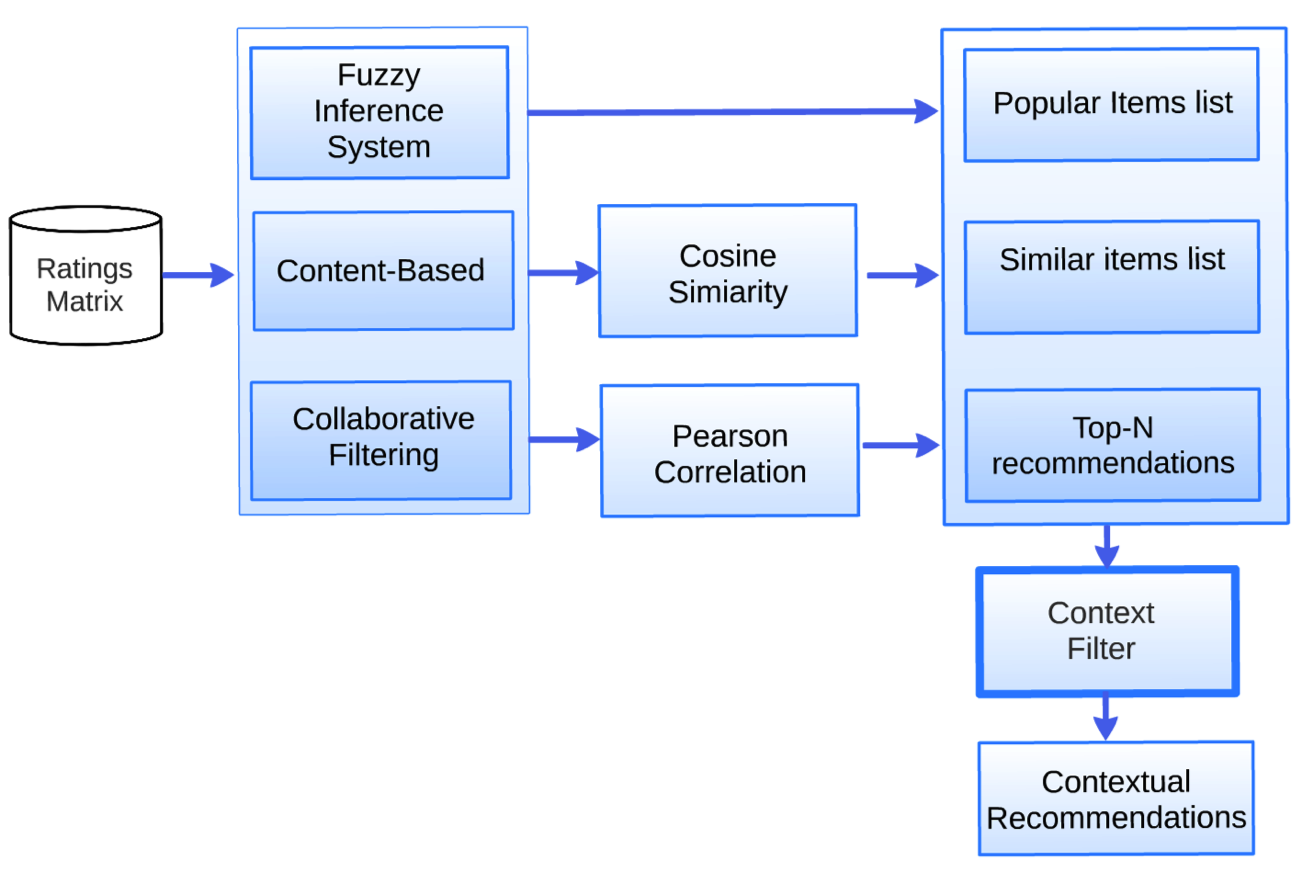
\includegraphics[width=0.80\textwidth]{img/archit-ta.png}
\caption{Recommender system methodology.}
\label{fig:architecture}   
\end{figure*}
Two tests were performed using TripAdvisor dataset, 
Table  \ref{tab:3} describes the data sets and the scarcity percentage of the
specified data. \\ Scarcity of 99\% mean that there are problems to
recommend items because the information is not enought to get 
good recommendations.
\begin{table}
\centering
\small
\captionsetup{font=footnotesize}
\caption{Datasets description.}
\label{tab:3}      
\begin{tabular}{lllll}
\hline\noalign{\smallskip}
Dataset & Users & Items & Ratings & Scarcity (percent) \\
\noalign{\smallskip}\hline\noalign{\smallskip}
TripAdvisor v1 & 1202 & 1890 & 4669 & 99.79 \\
TripAdvisor v2 & 2731 & 2269 & 14175 & 99.77 \\
\noalign{\smallskip}\hline
\end{tabular}
\end{table}
By other side, in Table  \ref{tab:4} the comparison
shows that the algorithm has a acceptable performance, i.e., the error
falls into the range of results obtained with others algorithms. 

\begin{table}
\centering
\small
\captionsetup{font=footnotesize}
\caption{Comparison of root mean square error.}
\label{tab:4}  
\small   
\begin{tabular}{lll}
\hline\noalign{\smallskip}
Dataset & Algorithm & Error \\
\noalign{\smallskip}\hline\noalign{\smallskip}
TripAdvisor v2 & collaborative filtering + Post-filtering  & 0.504  \\
                        & collaborative filtering                           & 0.994  \\
                        & Pre-filtering + Relaxation                     & 0.985  \\
\noalign{\smallskip}\hline
\end{tabular}
\end{table}
Then, contextual recommendations were evaluated with the 
root mean square error in order to compare the results with context 
relaxation algorithm  \cite{zheng2012differential} that is evaluated 
with the same dataset.\\ 
The cosine similarity plays an important role in content-based because
if similarity value among items is high, the recommendations will
improve the degree of user satisfaction. This is observed when
calculating the similarity average in each dataset as shown in 
Table  \ref{tab:5}.\\ 
Fuzzy inference system can provides a list of popular items for each dataset,
recommendations through averages obtained, and recommendations are
conditioned to show it when the collaborative filtering and content-based 
are not delivering recommendations because of data scarcity.
However, the majority of popular items of dataset were rated in contexts: 
\textit{romantic, family and bussines}, that means that the dataset has
biases that affects the results.

\begin{table}
\centering
\small
\captionsetup{font=footnotesize}
\caption{Level of similarity among items in datasets. }
\label{tab:5}      
\begin{tabular}{lll}
\hline\noalign{\smallskip}
Dataset  & Similarity  & Avg.votes per user. \\
\noalign{\smallskip}\hline\noalign{\smallskip}
TripAdvisor v1 & 0.448  & 5  \\
TripAdvisor v2 & 0.508  & 8  \\
\noalign{\smallskip}\hline
\end{tabular}
\end{table}

\section{Context-aware recommender system prototype} 

This section presents a context-aware recommender system prototype.
The backend have been explained in chapter  \ref{method},  in sections
 \ref{restaurants} and  \ref{hotels} talk about experiments realized
using the recommendation techniques proposed. \\ To develop the prototype
was used python language, technologies as Django Framework 1.7,
JavaScript, JQuery, Ajax, HTML5, Bootstrap 3.0  and PotsgreSQL for database.\\ 
Some dependencies and libraries were used also, it can review links of
downloads in appendix  \ref{appendixa}.

\subsection{User Interfaces}

The system starts in a landing page, the user should do \textit{Sign in} or
\textit{Sign up} to create a new user to enter the home page. \\ 
Landing page contains the \textit{Best restaurants} rated and 
\textit{Featured top list restaurants}
proposed by users, such as shows it the Figure  \ref{fig:landing}, 
the restaurants are updated while users add ratings, 
if the tendency is changed, the section displays the change 
in the tendency. \\ The aim is to provide
information for old and new users,the prototype tries to keep updated
the current preferences of users constantly.
\begin{figure*}
\captionsetup{font=footnotesize}
\centering
\fbox{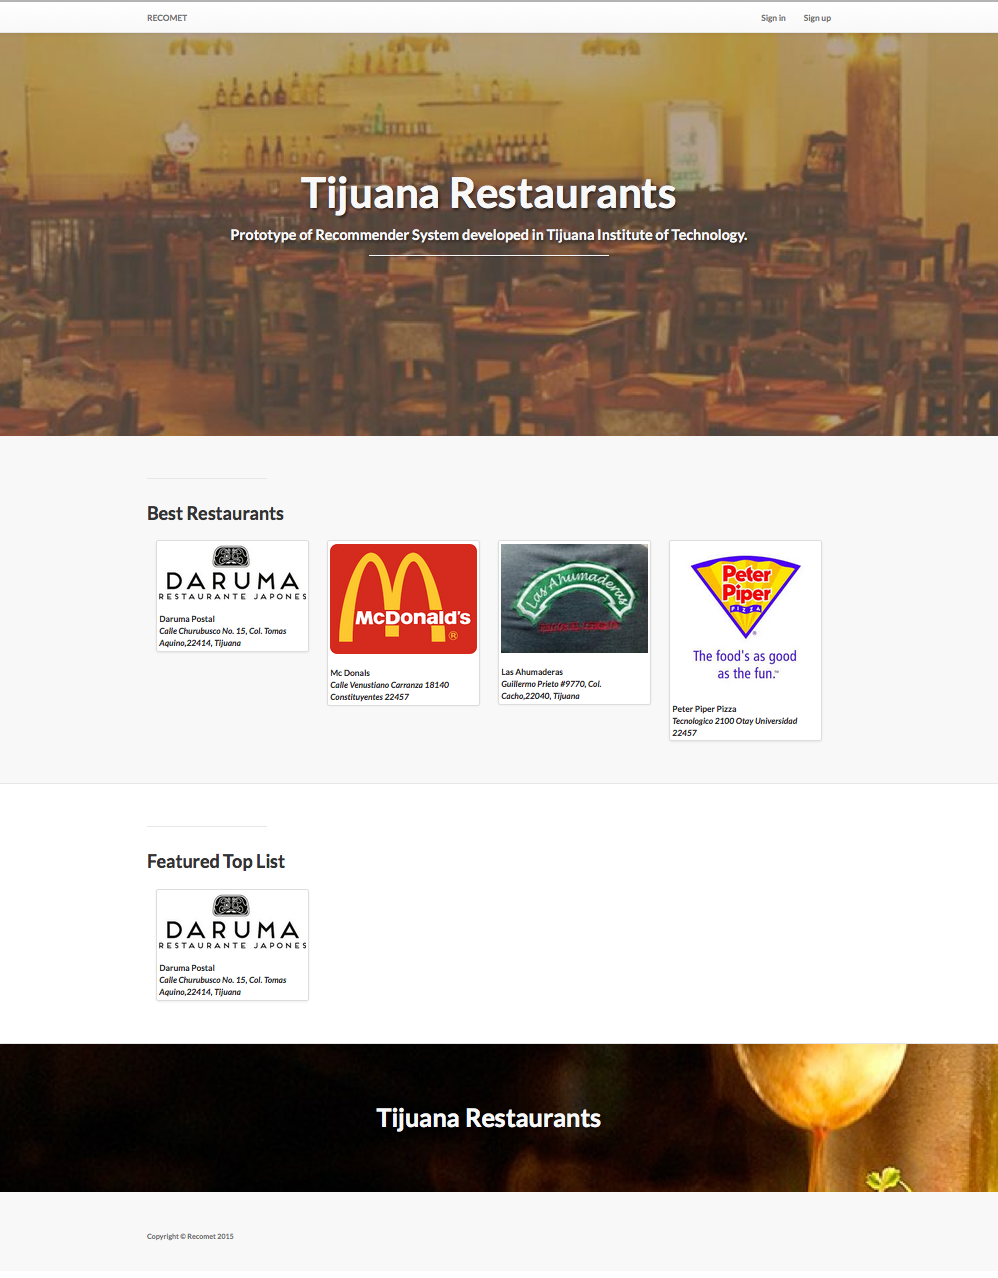
\includegraphics[width=0.60\textwidth]{img/landingpage.png}}
\caption{Landing page interface.}
\label{fig:landing}   
\end{figure*}

\subsubsection{Home Page interface}

\begin{figure*}
\captionsetup{font=footnotesize}
\centering
\fbox{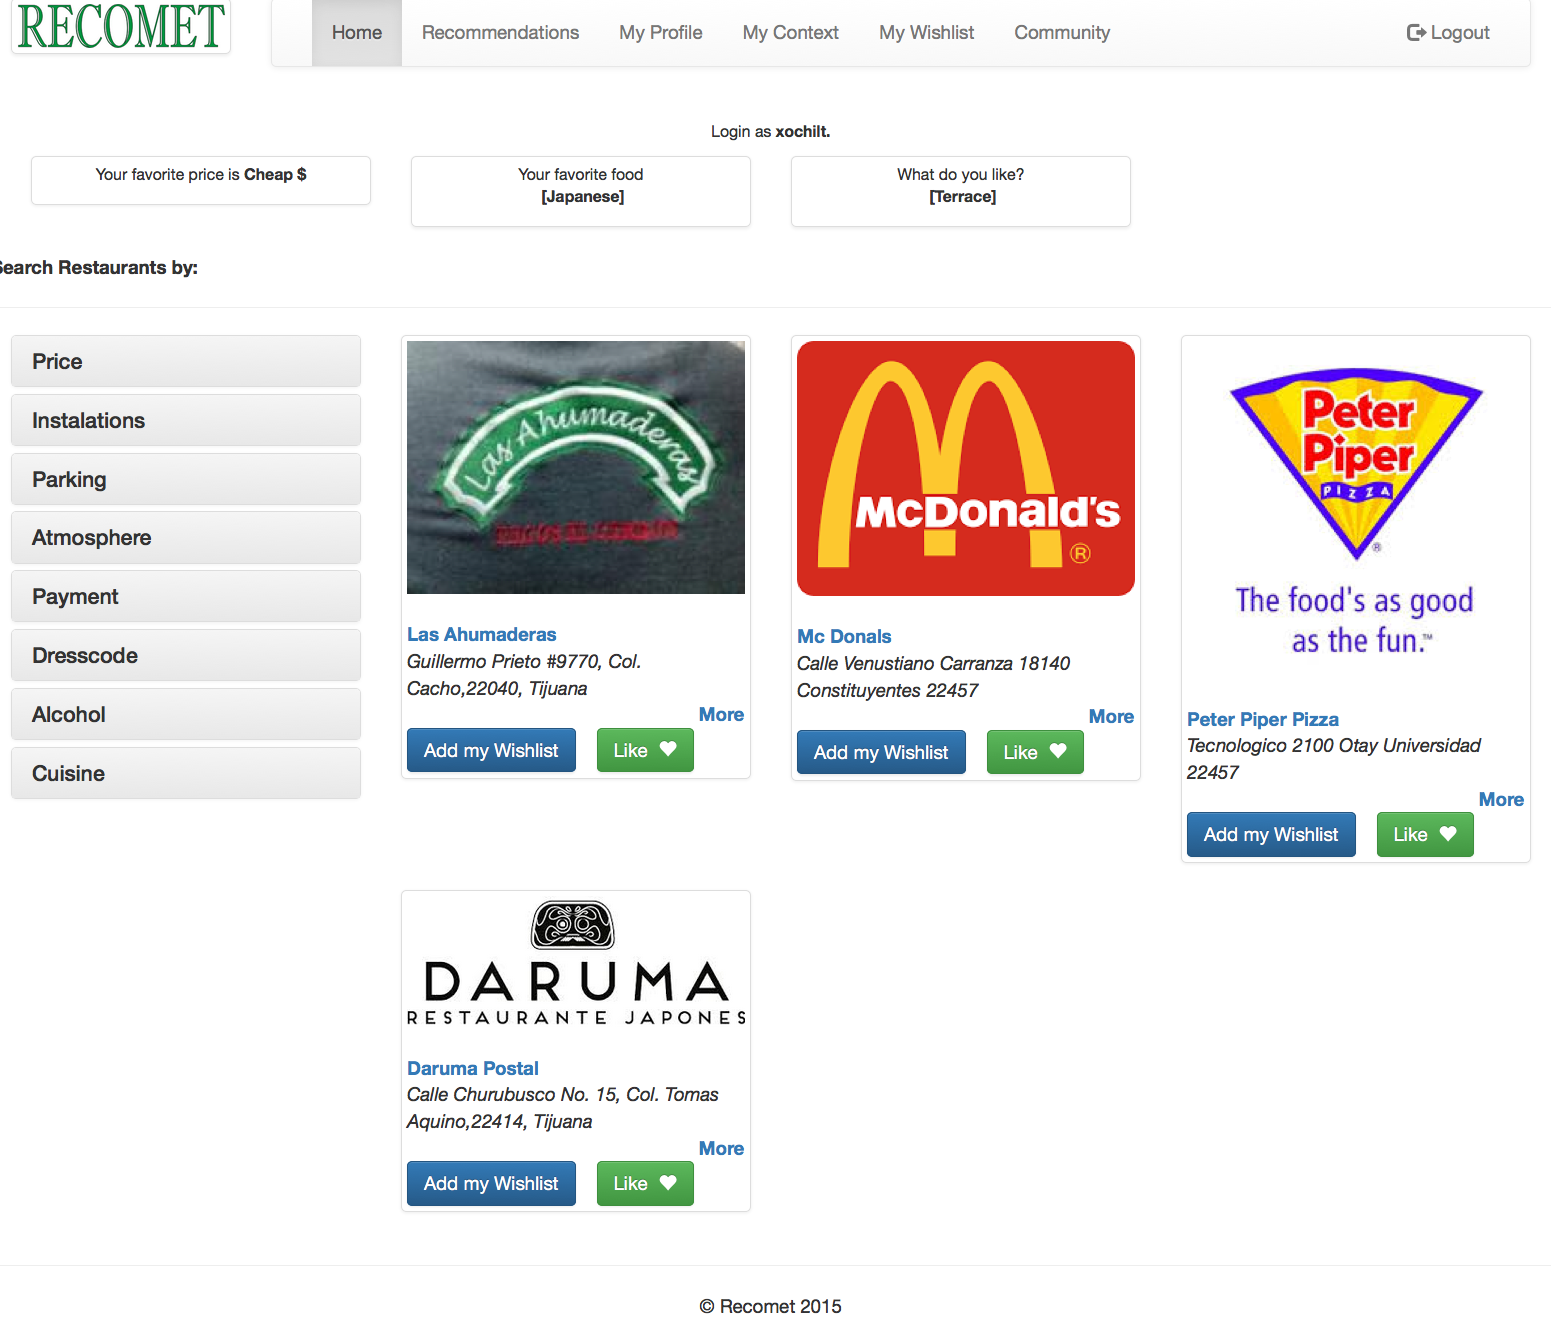
\includegraphics[width=0.60\textwidth]{img/homepage.png}}
\caption{Home page interface.}
\label{fig:home-page}   
\end{figure*}
\textit{Home Page} (Figure  \ref{fig:home-page}), shows the main
menu, tags for user preferences, all filters to start the search of
restaurants and the most popular restaurants in the community. \\ 
Users can start exploring filters to find restaurants under their own
criteria, each restaurant has a profile with complete information
about the characteristics and opinions of other users. \\ When users
click the restaurant picture the system redirects to the profile, for
instance Figure  \ref{fig:rest-profile2}  shows the profile of Daruma
restaurant, the Figure  shows the general information of the
restaurant, reviews or personal opinions of users that visited the
restaurant, details about ratings, the chart of ratings and the user
location using Google maps services. It is also added the button to
\textit{add wishlist}, this element will be explained in a posterior
section.
\begin{figure*}
\captionsetup{font=footnotesize}
\centering
\fbox{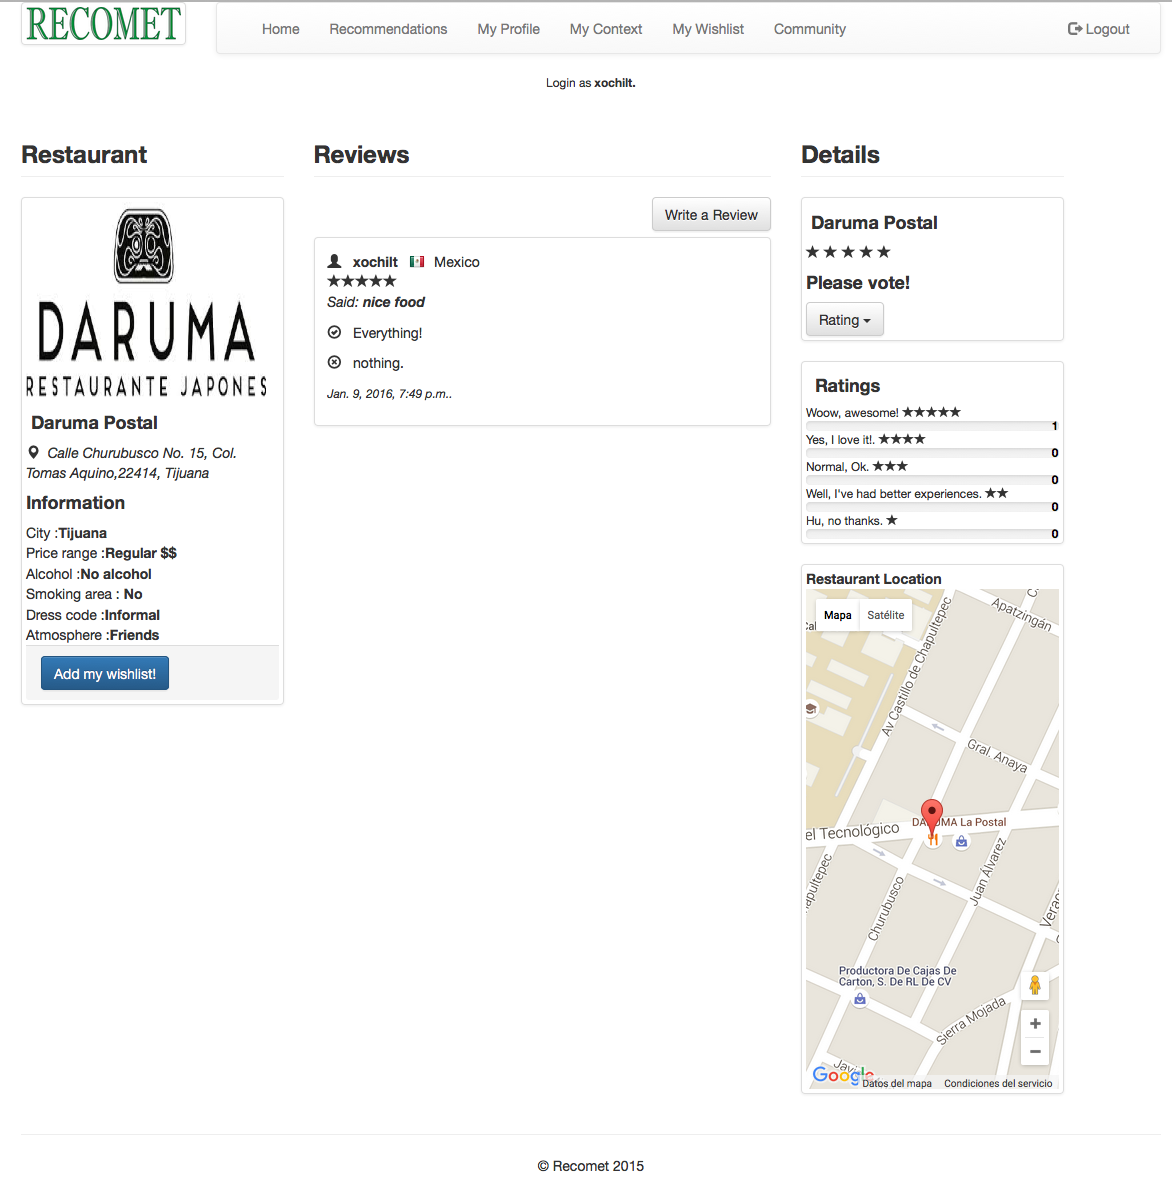
\includegraphics[width=0.60\textwidth]{img/rest-profile.png}}
\caption{Restaurant profile interface.}
\label{fig:rest-profile2}   
\end{figure*}

\subsubsection{My Recommendations interface}

\begin{figure*}
\captionsetup{font=footnotesize}
\centering
\fbox{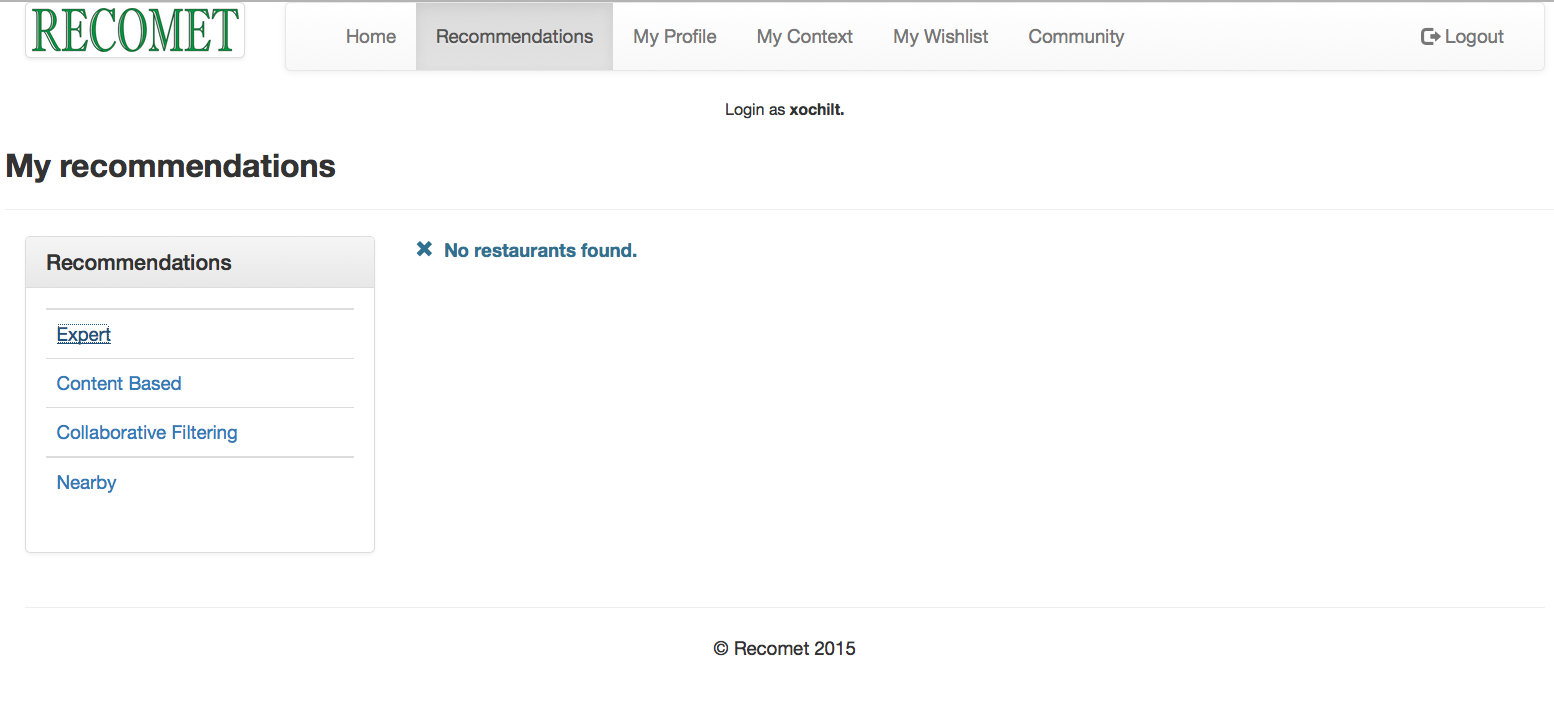
\includegraphics[width=0.60\textwidth]{img/expert-recs.png}}
\caption{Expert recommendations interface.}
\label{fig:expert-recs}   
\end{figure*}
In recommendations interface users have the options to get  
recommendations such as was described in chapter \ref{method}, four 
recommendation techniques works to suggest restuarants for 
users. Here, users can choose the prefered option to get 
information in the screen.\\ 
For instance, Figure \ref{fig:expert-recs} shows that the expert can 
not to recommend whether users don’t have participations, because of expert's
recommendation is based in fuzzy rules that involves the popularity of
items (input variable), if the information is sparse the prototype can
not get results and only shows an alert message. On the contrary case,
it shows a list of popular restaurants.
\begin{figure*}
\captionsetup{font=footnotesize}
\centering
\fbox{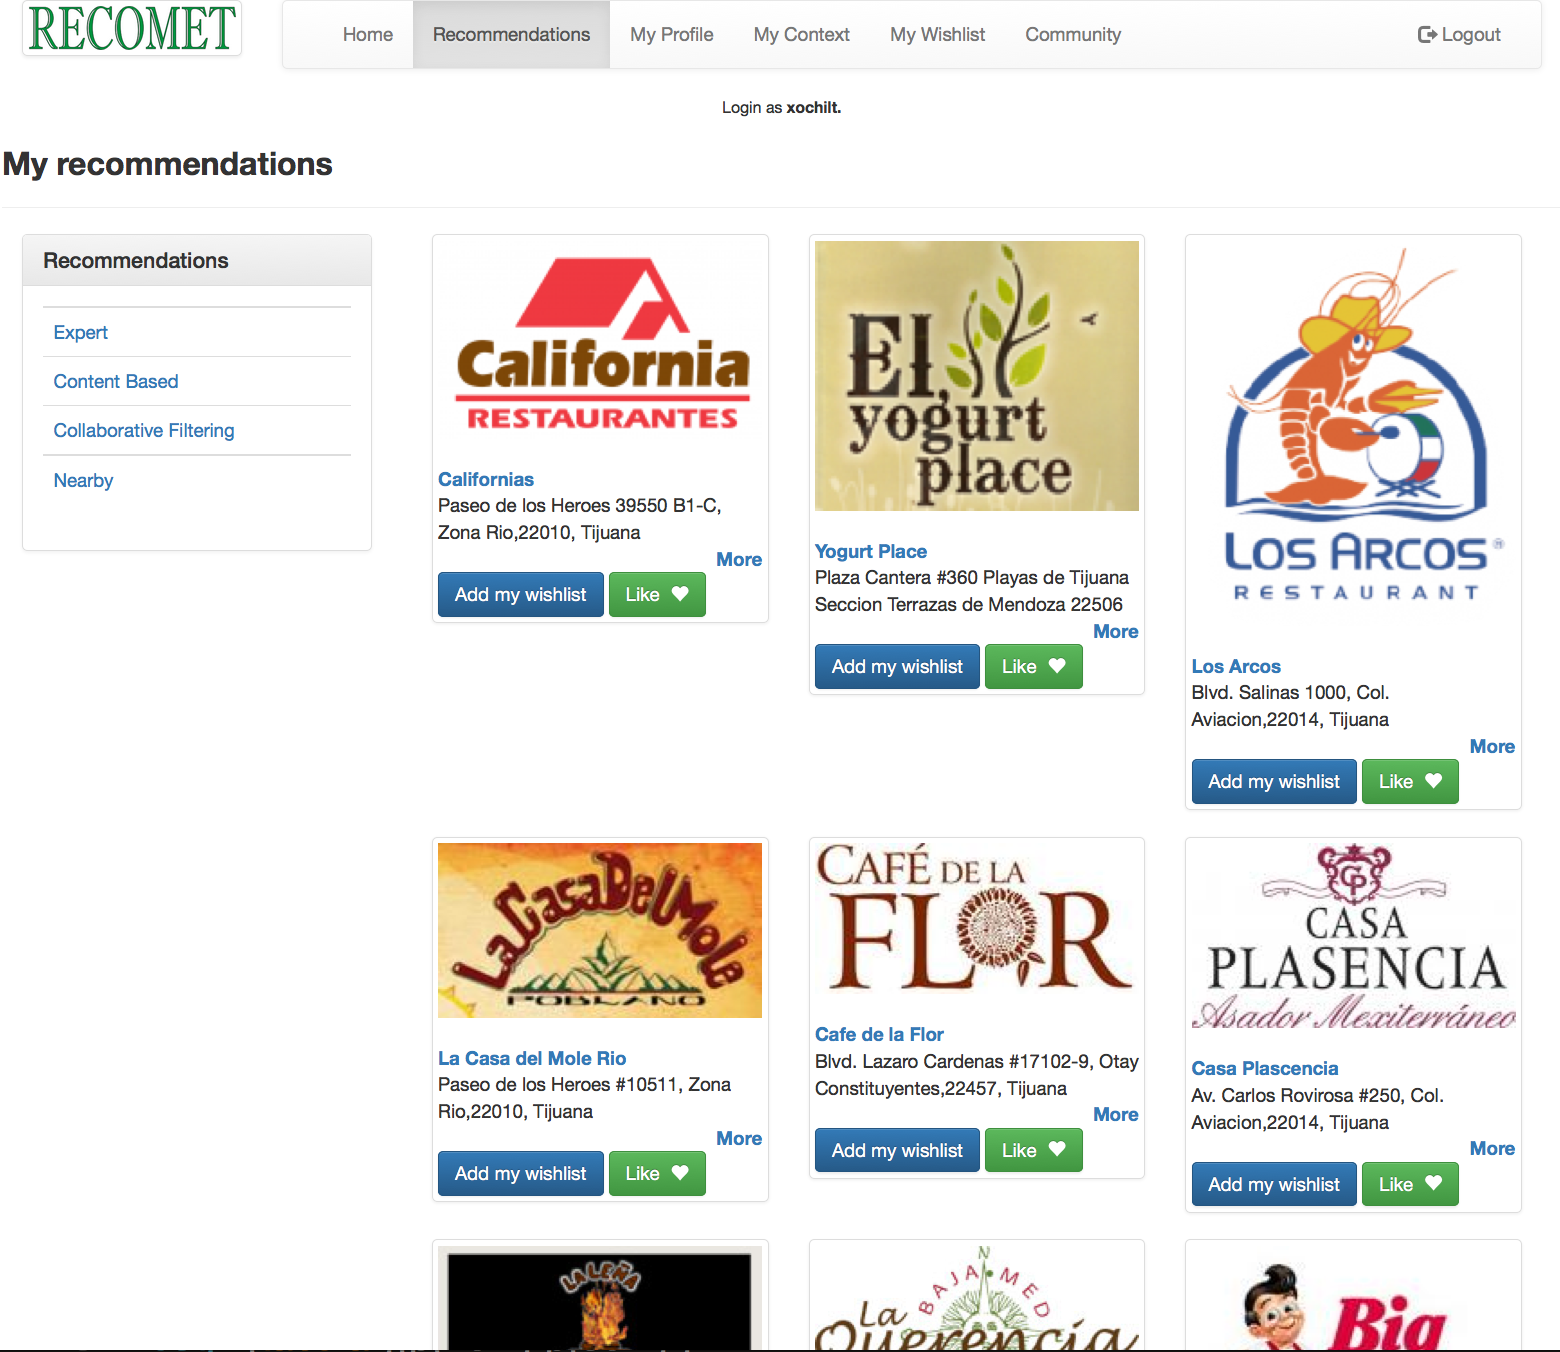
\includegraphics[width=0.60\textwidth]{img/base-content.png}}
\caption{Content-based recommendations interface.}
\label{fig:base-content}   
\end{figure*}
\\ \textit{Content-based recommendation} finds the similar restaurants to the
favorites of the user. In fact, makes a comparison of all restaurants
and gets the more similars to display in the screen. \\
Figure \ref{fig:base-content}  
shows the results of the search, large amount of restaurants are showed
because of the similarity among restaurants, this is the most
efficiently way to get recommendations when the system has not enough
information about user preferences and it the users community is
small. It is not functional whether the user has not at less one vote
with high rating (five stars).\\
\textit{Collaborative filtering recommendation} is depicted in the 
Figure  \ref{fig:cf-recs}
this technique is based in users' opinions, if the system has not
information of users, or whether the users community is small, 
cold-start problem highlights in results. 
\begin{figure*}
\captionsetup{font=footnotesize}
\centering
\fbox{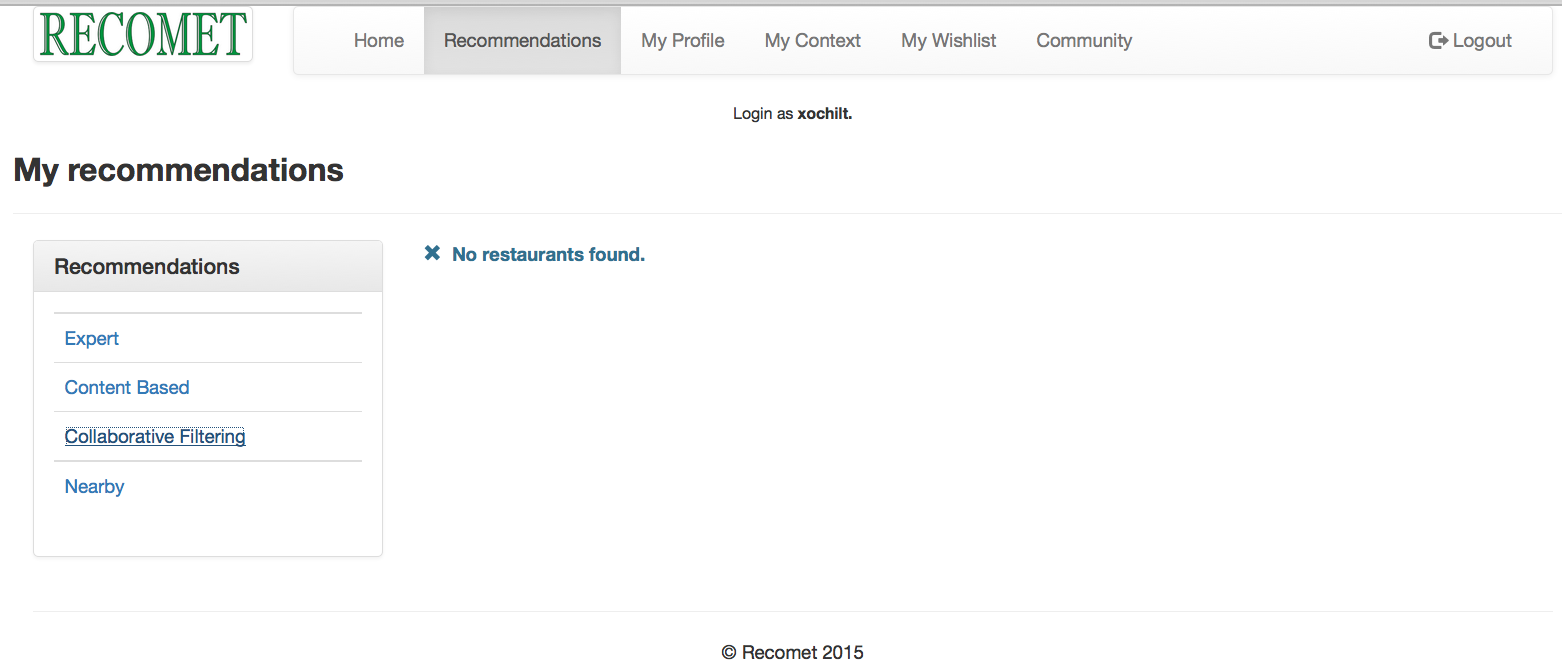
\includegraphics[width=0.60\textwidth]{img/cf-recs.png}}
\caption{Collaborative filtering recommendations interface.}
\label{fig:cf-recs}   
\end{figure*}
\begin{figure*}
\captionsetup{font=footnotesize}
\centering
\fbox{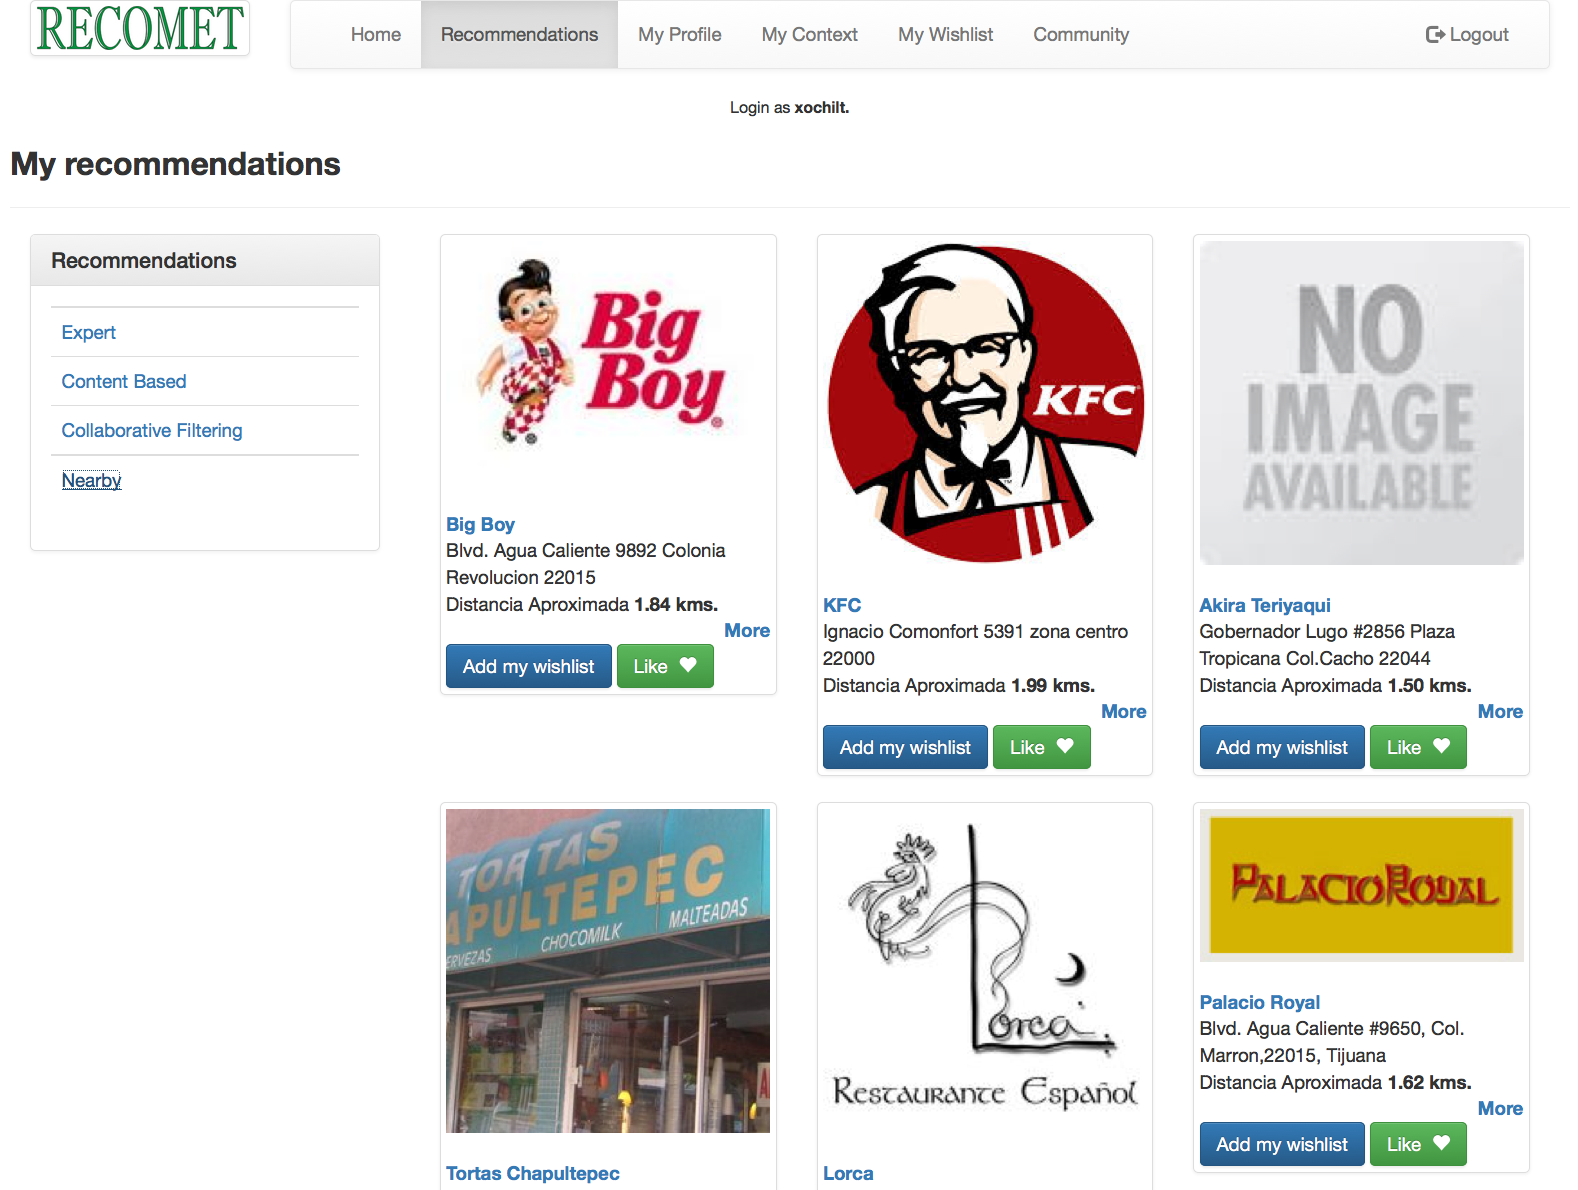
\includegraphics[width=0.60\textwidth]{img/nearby-recs.png}}
\caption{Nearby recommendations interface.}
\label{fig:nearby-recs}   
\end{figure*}

As in expert  recommendations if the users participations 
is low or null, the results of recommendations will be empty 
and the alert message appears in the
screen, else, the restaurants suggested will be displayed 
in the screen.\\
\textit{Nearby recommendations} (Figure \ref{fig:nearby-recs}) 
provides recommendations when the
user previously specifies a geographical position. The distance to
considers restaurants from the current position to two kilometers
around. Then, recommendations are displayed in the screen if the
location is provided in the context, else, an alert message  notifies
the lack of user current location.

\subsubsection{My Profile interface}

\begin{figure*}
\captionsetup{font=footnotesize}
\centering
\fbox{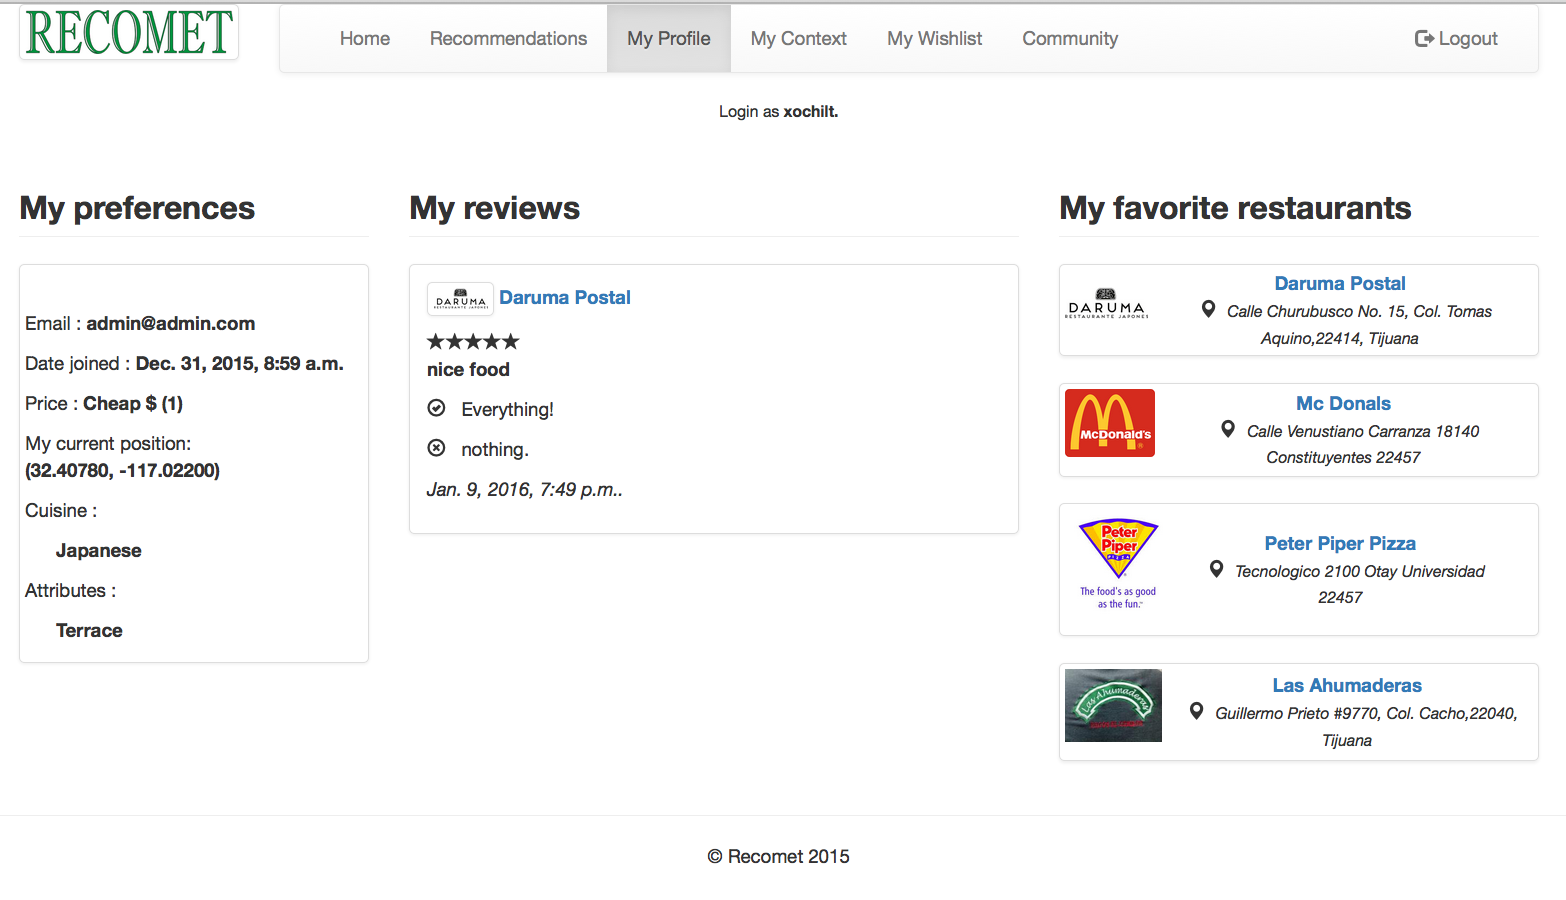
\includegraphics[width=0.60\textwidth]{img/myprofile.png}}
\caption{My Profile interface.}
\label{fig:myprofile}   
\end{figure*}
My Profile interface shows all the information of the user divided in
three sections: my preferences, my reviews and my favorite restaurants
as shown in Figure  \ref{fig:myprofile}. \\ The preferences represent the basic
information and tastes of a user, it contains the tastes and preferences
of the user, some factors as price, position, cuisine and attributes
of restaurants could be changing continuosly, it depends how the user
want manage its information.\\ The prototype uses this information every
time that a request of recommendation is done.
The My reviews section shows all the reviews that the user typed, each
review is stored in database and the user cannot delete it. \\ The stars
represent the level of satisfaction of the user when he/she visits the
restaurant, each review highlights the good and the bad things that
the user perceives in the visit. \\ This information is valuable but,
unfortunatly this prototype not uses it to infer possible tastes and
preferences and subsequently, recommendations. This process might be a
functionality integrated in the future.\\
My favorite restaurants section, displays restaurants rated with five
stars. It means that are the more important options of the user to
visit in this moment and in the future. These restaurants are related
to the content-based recommendation because are the restaurants with
high rating of this particular user.

\subsubsection{My Context interface}

My Context interface is divided in two sections: contextual 
information and current location as in the Figure  \ref{fig:mycontext}.
Contextual information represents the user preferences, for instance
the price range that wants for a specific ocasion, the attributes are
the characteristics of restaurants, so it selects as many as the user
prefers, the limit is the number of characteristics displayed. 
 \begin{figure*}
\captionsetup{font=footnotesize}
\centering
\fbox{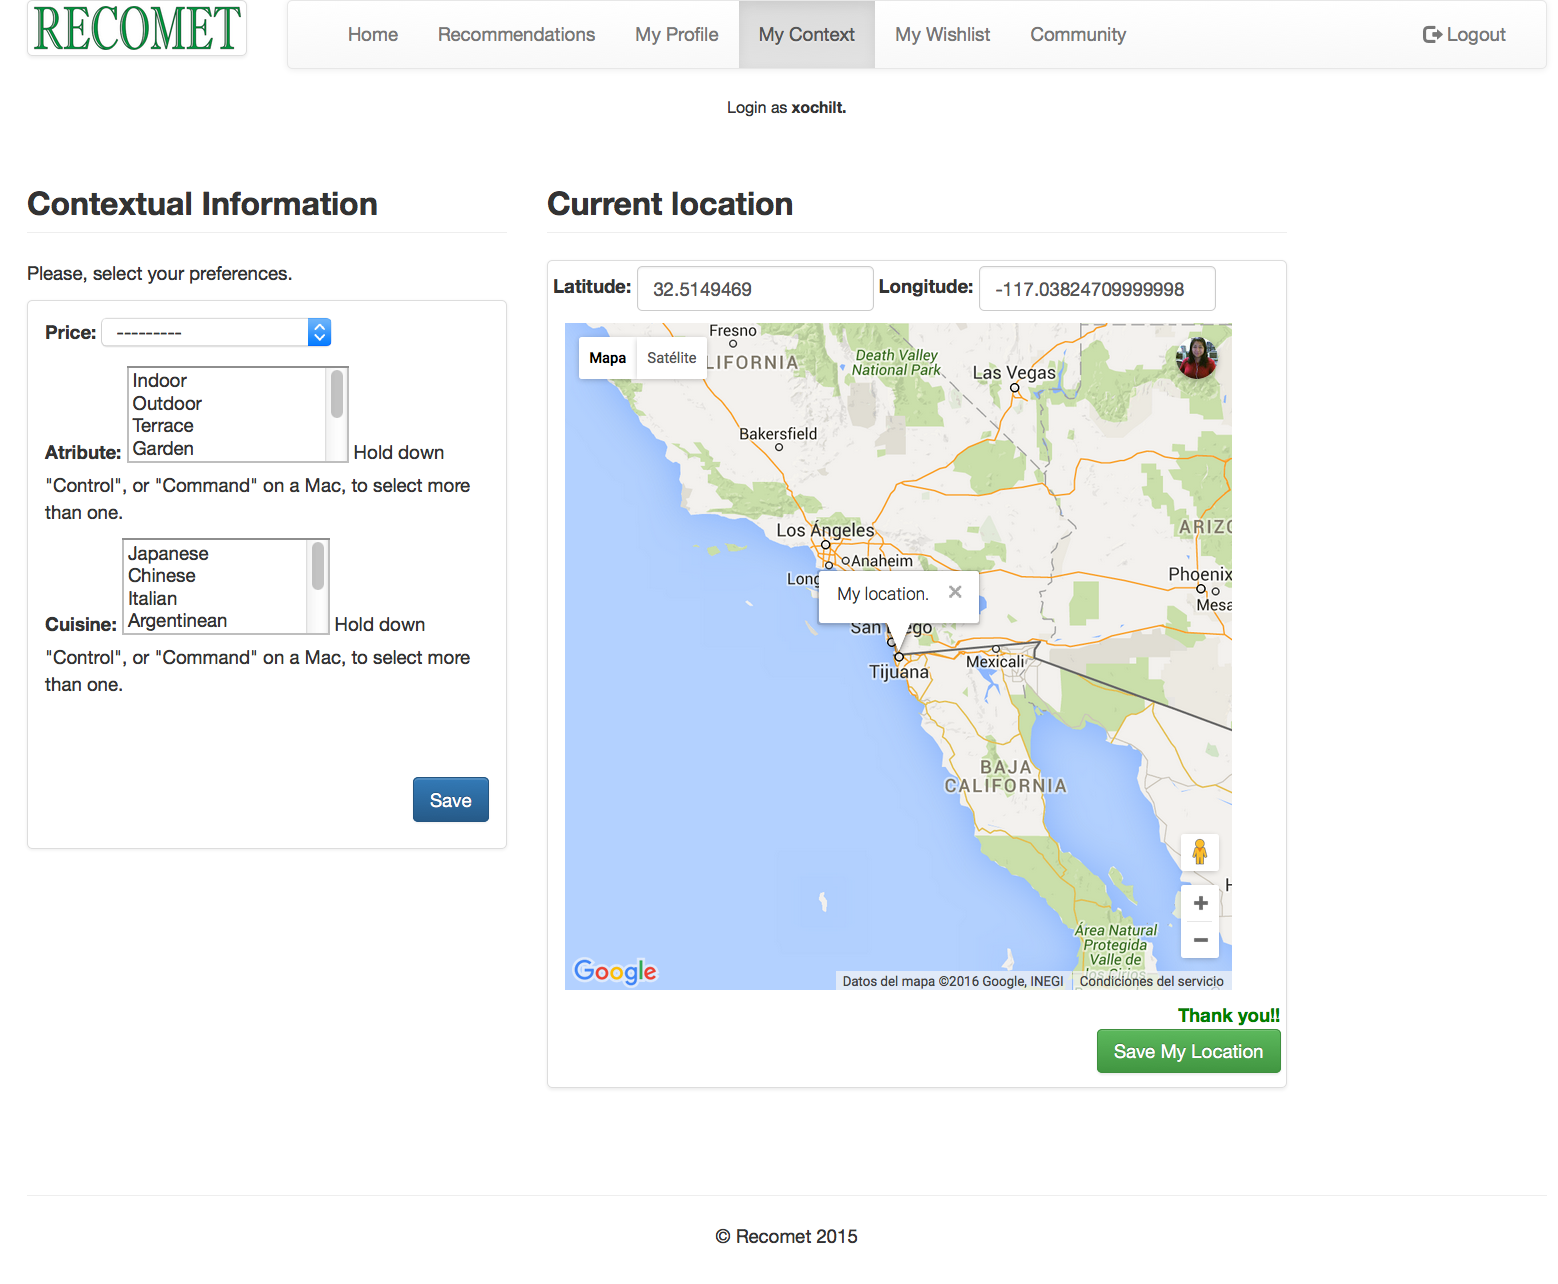
\includegraphics[width=0.60\textwidth]{img/mycontext.png}}
\caption{My Context interface.}
\label{fig:mycontext}   
\end{figure*}
\\ The same is for cuisines, a total of 30 type of cuisines were
proposed considering the list of restaurants in the prototype, it can
select as many as the user want.  \\All this information is stored and
displayed in home page also in order to help the user to remember
which is the information that the prototype is using to display
recommendations.\\  Current location section shows the Google map to
display the current location, previously the user ought to confirm
that wants to share the current location. \\  When user click in the
\textit{Save My Location button}, the content in the box of latitude
and longitude will be stored in the database(alert message  confirms
the action) and the status will be modified when user location
changes, then, all the locations stored in database become user's
historical information.

\subsubsection{My Wishlist interface}

\begin{figure*}
\captionsetup{font=footnotesize}
\centering
\fbox{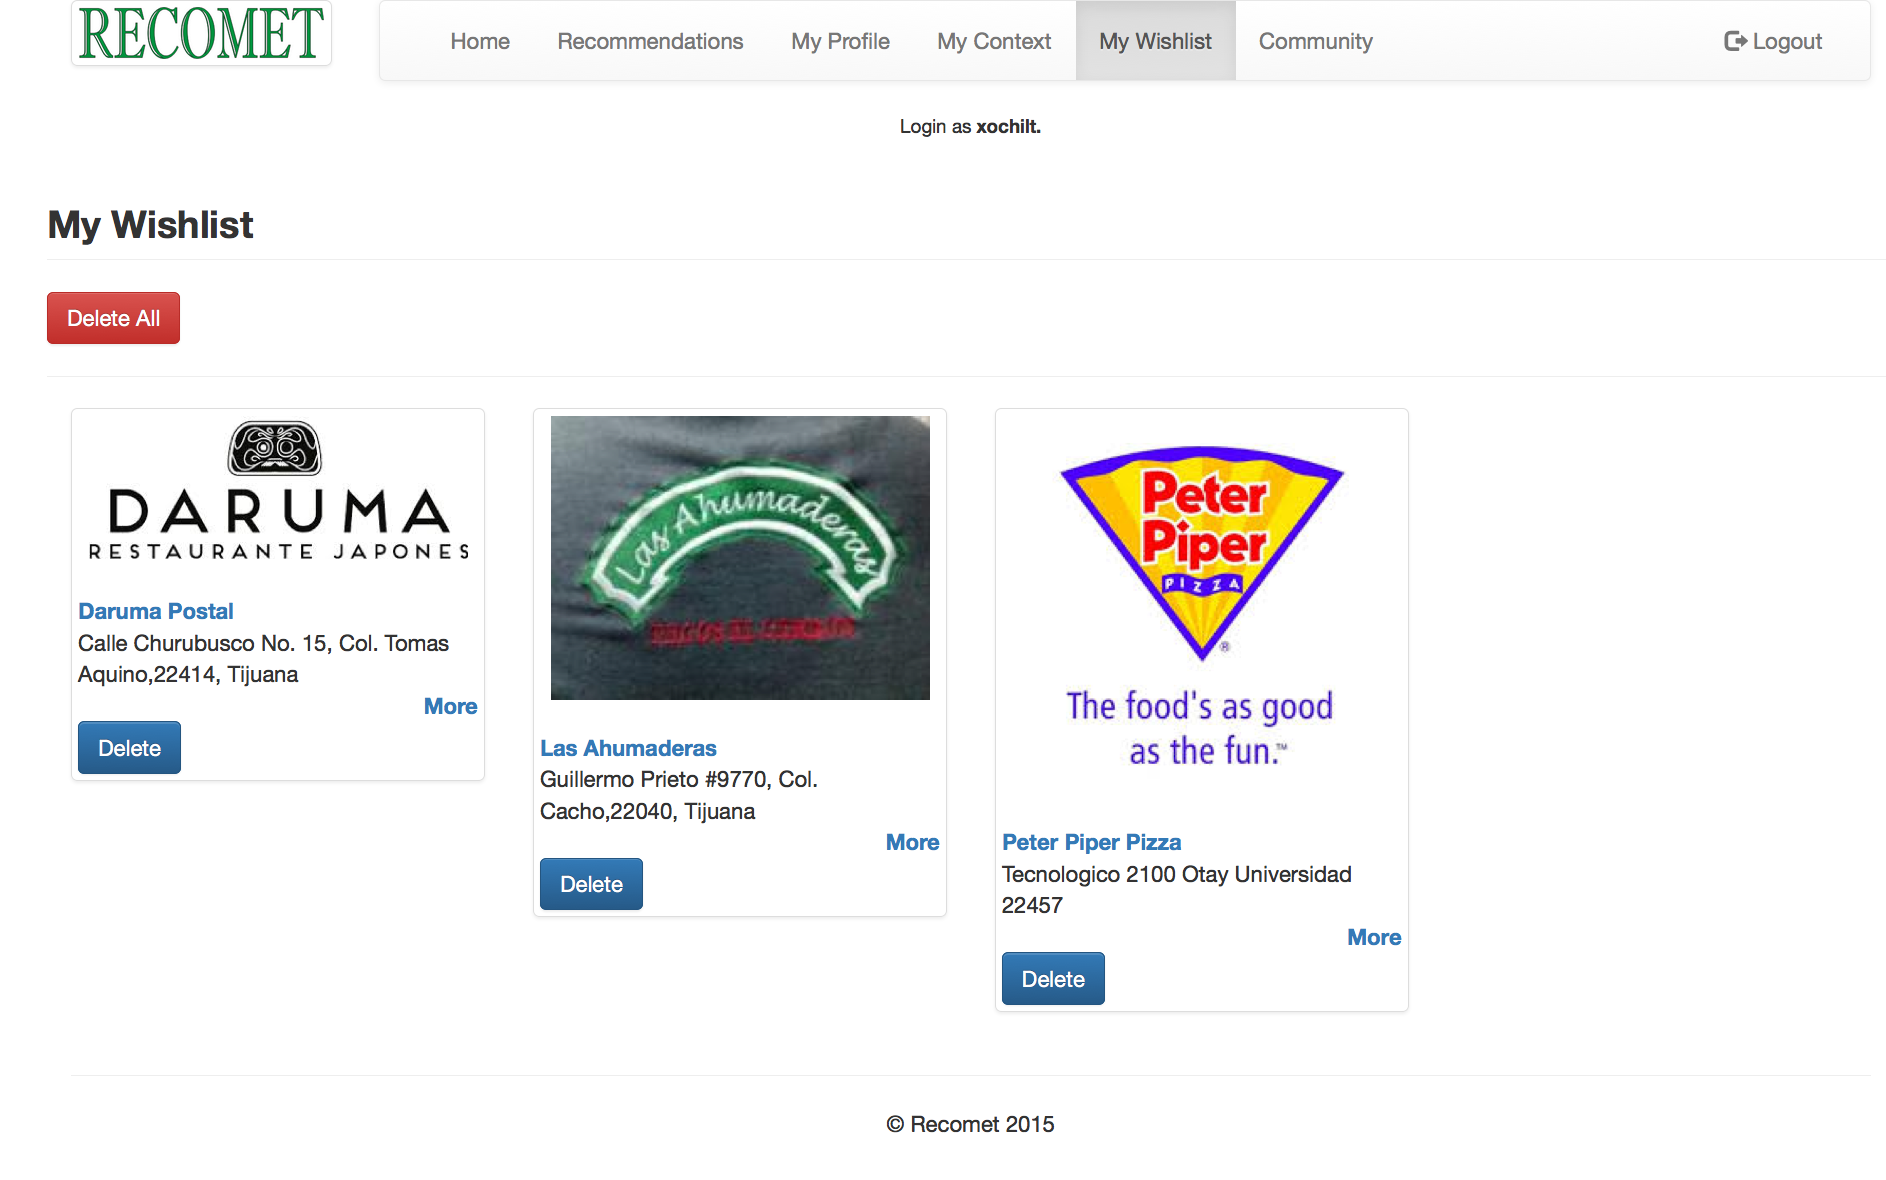
\includegraphics[width=0.60\textwidth]{img/mywishlist.png}}
\caption{My Wishlist interface.}
\label{fig:mywishlist}   
\end{figure*}
My Wishlist interface contains the restaurants that are  considered by
the user as future options to vist  (Figure  \ref{fig:mywishlist})  or
simply to have available information for a particular  ocasion. \\The
wishlist allows the manipulation of restaurants,  it means, user can
add or delete restaurants as many as  he/she wants. \\The wishlist could
be empty or full of  restaurants, this information does not affect any
functionality  of the prototype. \\
Making a comparison with others platforms (for instance 
Amazone), this information allows the user to have the own 
\textit{personalized store}, in terms of products sales, the wishlist 
should be the future products to buy.\\ In a similar way, 
this prototype tries to infer the future tastes of the user 
or what restaurants could visit the user in a close future. \\
To facilitates the addition of restaurants the \textit{Add my wishlist} 
button was added in every restaurant of the home 
page (Figure  \ref{fig:wishlist-home}) and in restaurants 
profiles (Figure  \ref{fig:rest-profile2}).
\begin{figure*}
\captionsetup{font=footnotesize}
\centering
\fbox{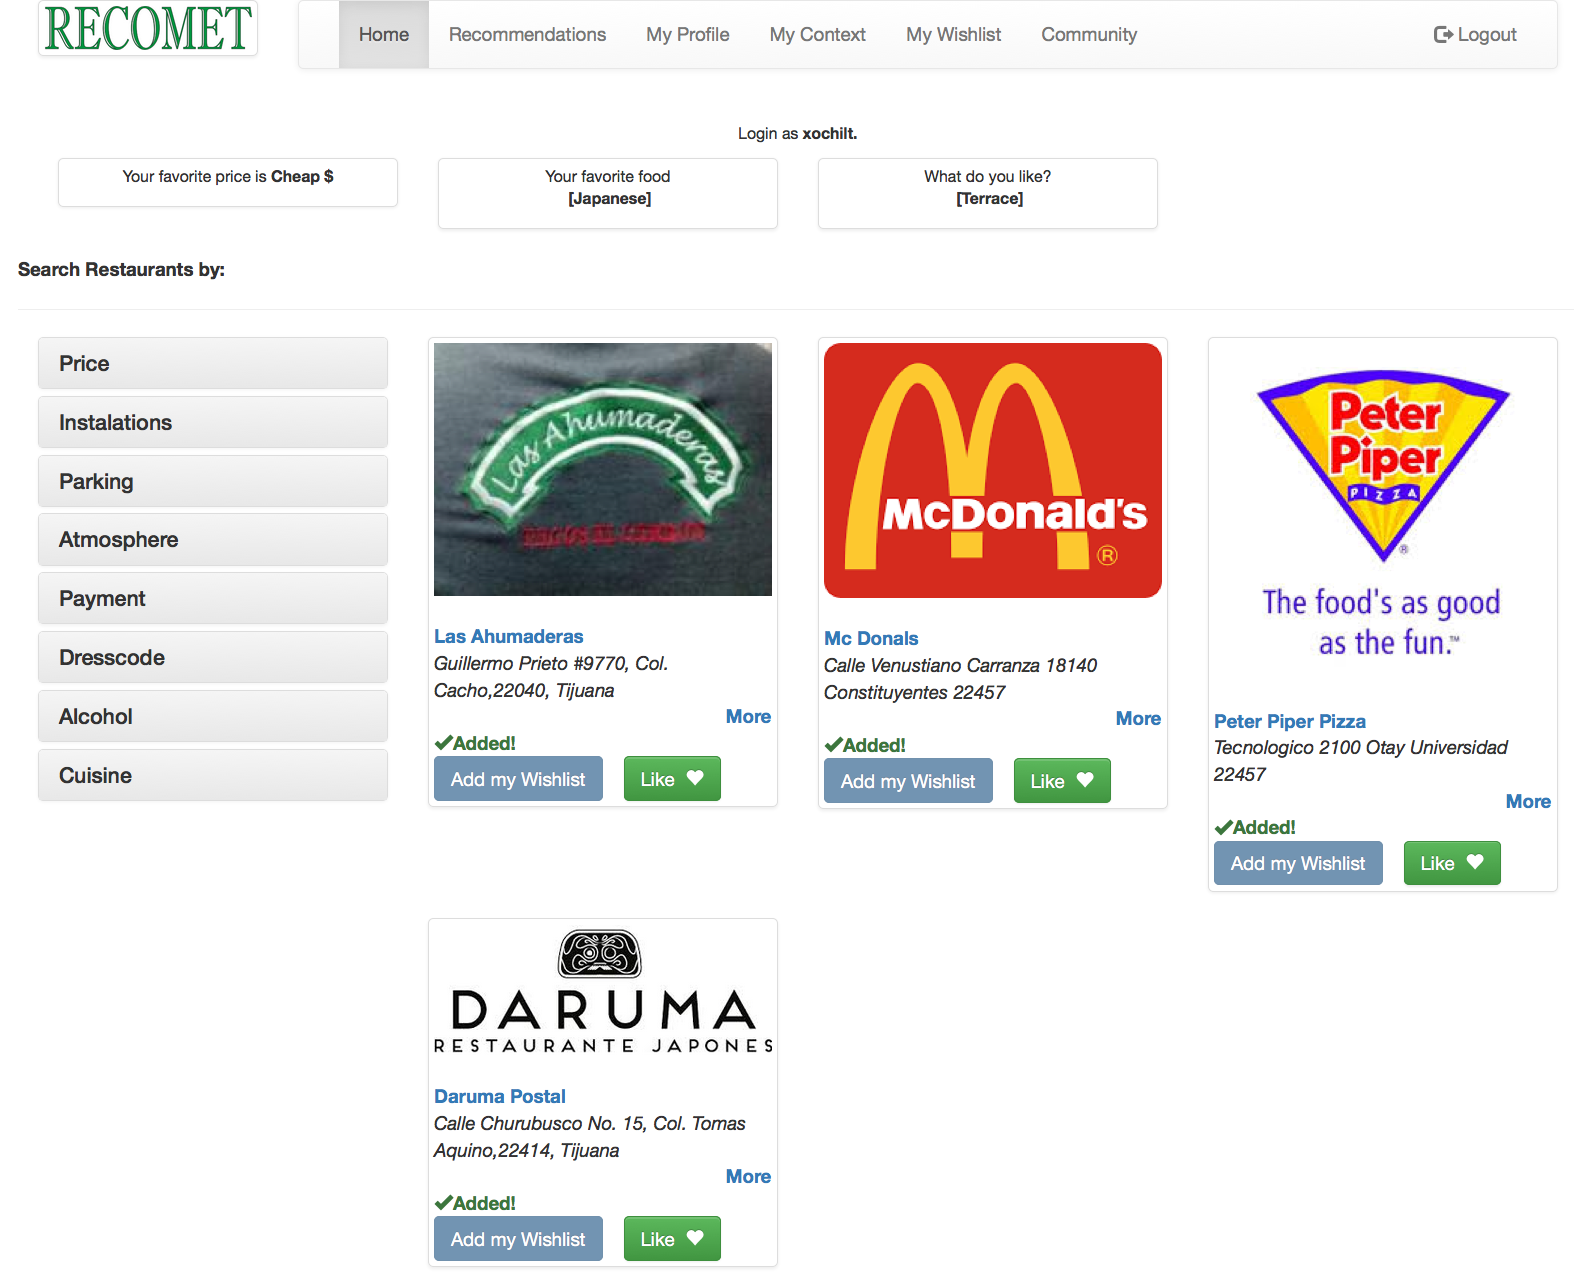
\includegraphics[width=0.60\textwidth]{img/wishlist-home.png}}
\caption{Functionality of wishlist button in Home page.}
\label{fig:wishlist-home}   
\end{figure*}

\subsubsection{Community interface}

The Community interface contains the reviews of all the users  
(Figure  \ref{fig:community}) in order to display information that may helps
another users to select any restaurant to visit. \\In the real life, the
persons recommend some or another restaurant in the common  language,
remarking the why the restaurant is good or bad according  their
perception. \\The Community section has the same goal, in fact,  some
reviews could be useful for the other users, this opinion may  express
it through the \textit{Helpful button}.
\begin{figure*}
\captionsetup{font=footnotesize}
\centering
\fbox{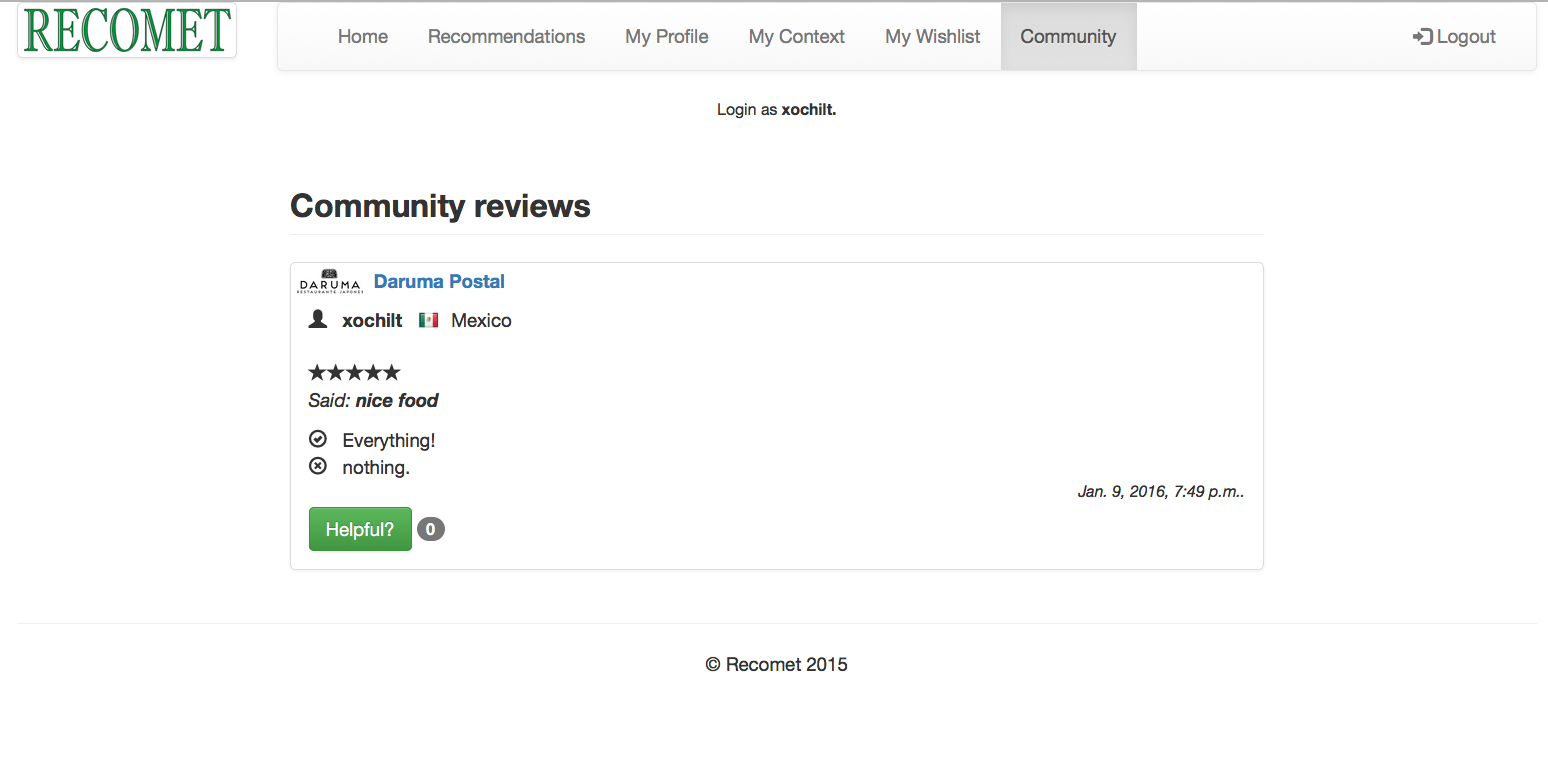
\includegraphics[width=0.60\textwidth]{img/community.png}}
\caption{Community interface.}
\label{fig:community}   
\end{figure*}
These are the functionalities in the prototype, in order to validate
the performance, an on-line experiment was realized, the metrics 
of usability applied were Time-taks and Taks-success (mentioned 
in chapter  \ref{introduction}). In the next chapter will be 
explained the tests and the results obtained.







